\section{教會及書信簡介}

\subsection{保羅去過的教會}

\begin{figure} 
\centering
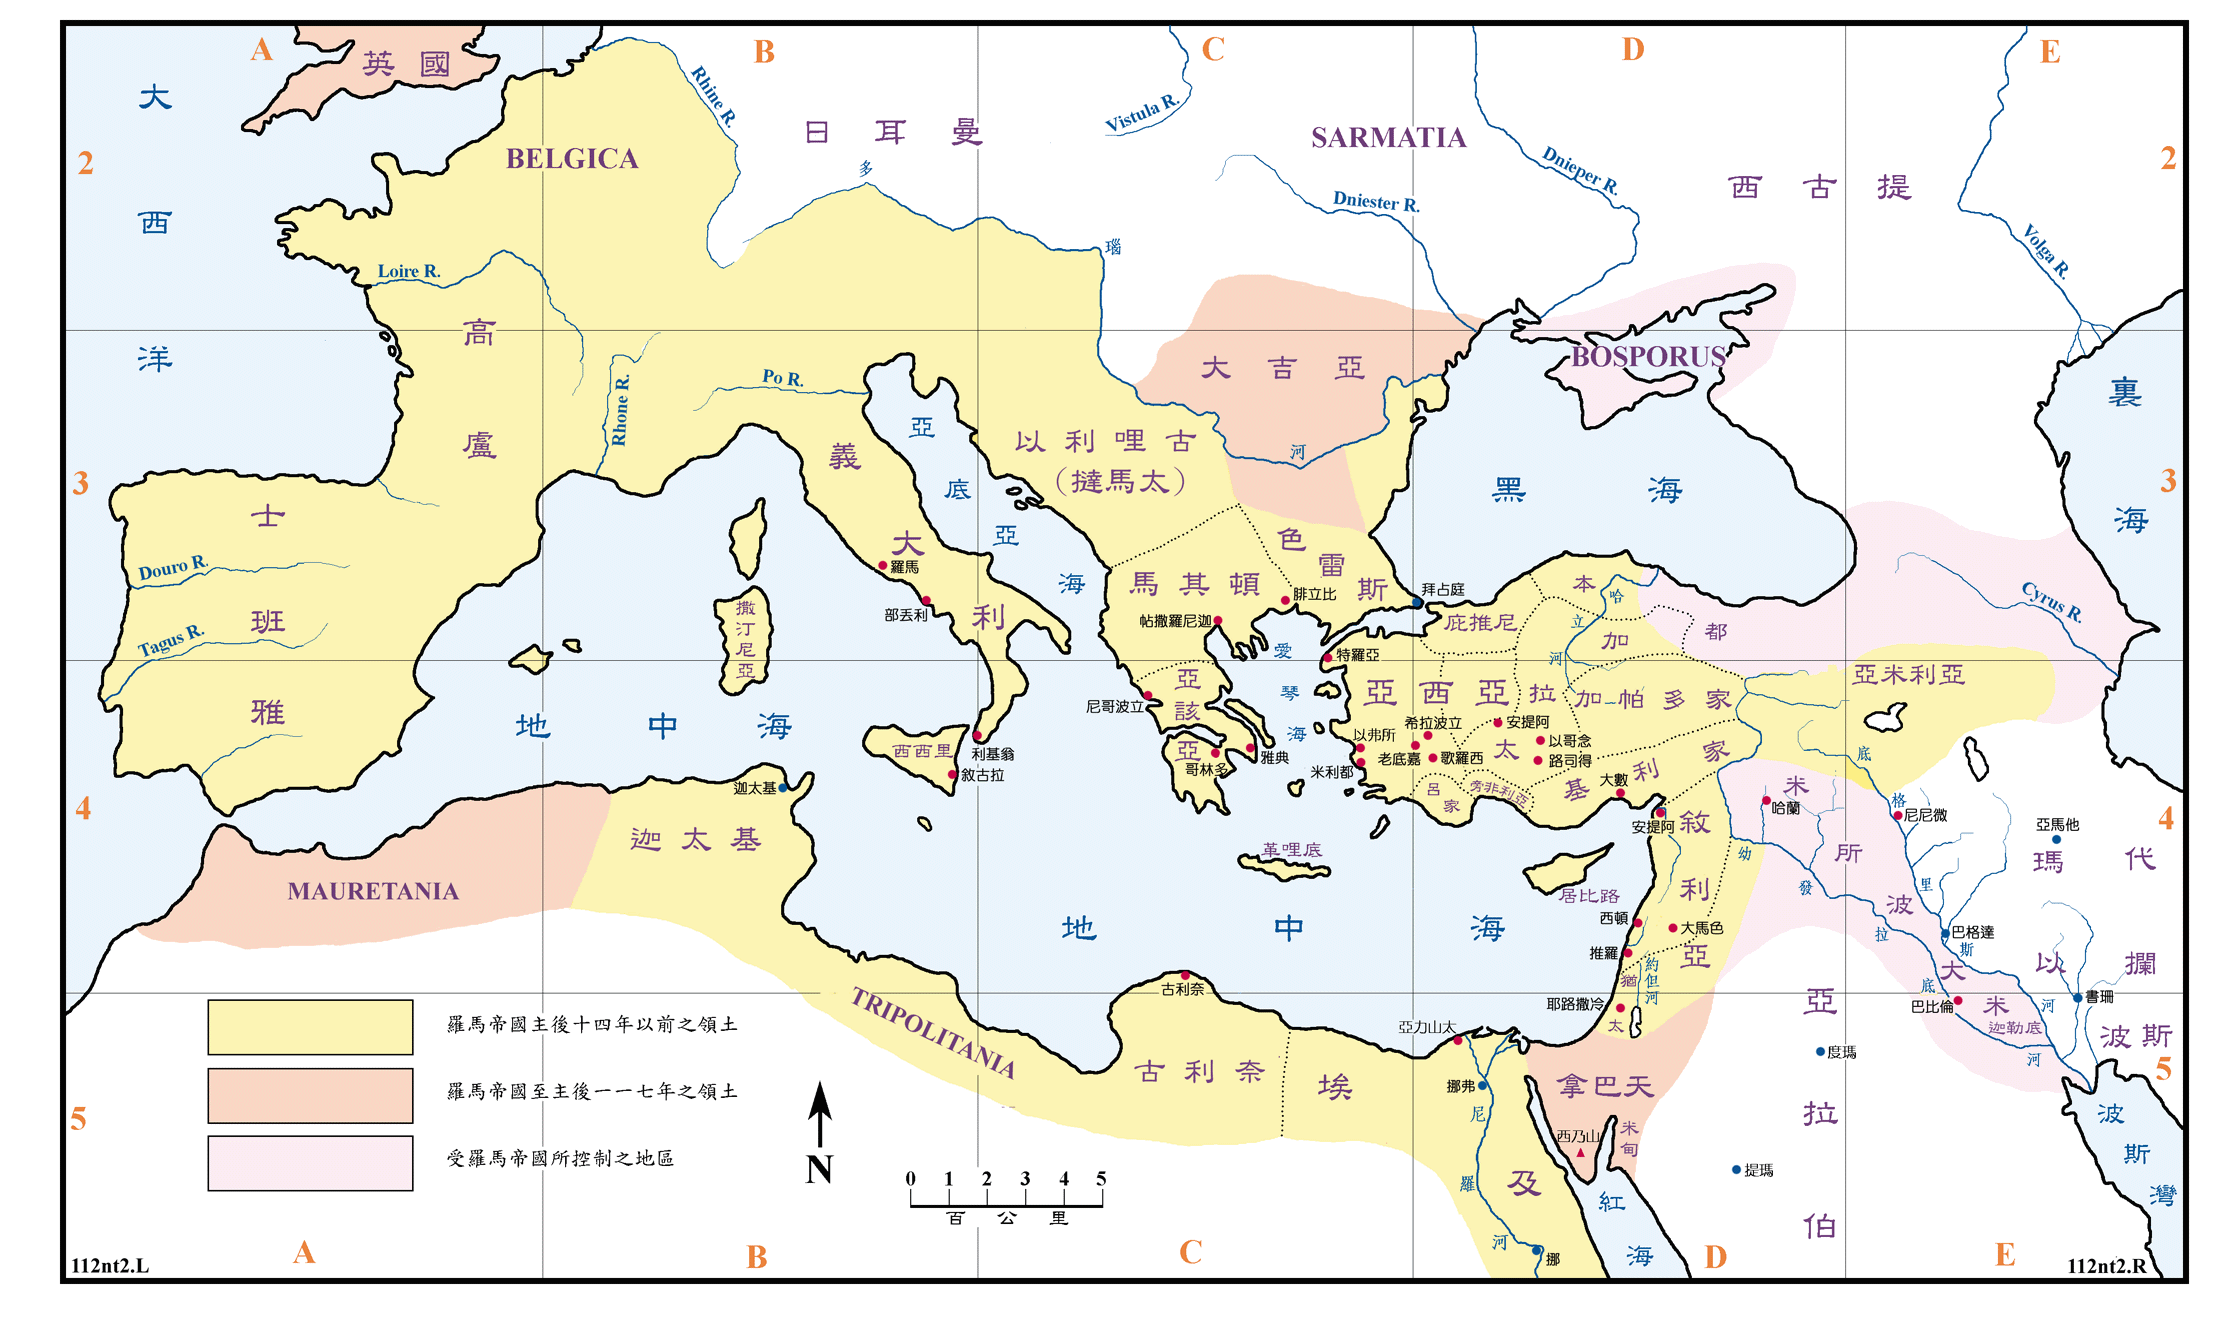
\includegraphics[width=7in]{Act/fig/church}
\caption{保羅去過的教會}
\label{fig:sub1}
\end{figure} 

\begin{table}[htbp]
  \centering
    \begin{tabular}{|l|l|l|l|}
    \toprule
   地區 &教會名字   &時間 &   經文\\
    \midrule   
   馬其頓& 帖撒羅尼迦   & 第二次宣教   &   \\
     \midrule
     馬其頓& 腓立比   & 第二次宣教   &   \\
     \midrule
     馬其頓& 庇哩亞   & 第二次宣教   &   \\    
    \bottomrule
    \end{tabular}%
      \caption{保羅去過的教會}
  \label{tab:addlabel}%
\end{table}%


\subsection{亞細亞教會}
\subsubsection{以弗所}
一，保羅與以弗所教會的關係
\begin{itemize}
\itemsep-.25em 
\item 保羅第二次宣教——徒18:18-28
\begin{itemize}
\itemsep-.25em 
\item 保羅\\
保羅又住了多日，就辭別了弟兄，坐船往敘利亞去，百基拉、亞居拉和他同去。他因為許過願，就在堅革哩剪了頭髮。 19 到了\textcolor{red}{以弗所}，保羅就把他們留在那裡，自己進了會堂和猶太人辯論。 20 眾人請他多住些日子，他卻不允， 21 就辭別他們，說：「神若許我，我還要回到你們這裡。」於是開船離了\textcolor{red}{以弗所}。 22 在愷撒利亞下了船，就上耶路撒冷去問教會安，隨後下安提阿去。 23 住了些日子，又離開那裡，挨次經過加拉太和弗呂家地方，堅固眾門徒。
\item 亞波羅、百基拉、亞居拉\\
有一個猶太人名叫亞波羅，來到\textcolor{red}{以弗所}。他生在亞歷山大，是有學問(口才)的，最能講解聖經。 25 這人已經在主的道上受了教訓，心裡火熱，將耶穌的事詳細講論教訓人，只是他單曉得約翰的洗禮。 26 他在會堂裡放膽講道，百基拉、亞居拉聽見，就接他來，將神的道給他講解更加詳細。 27 他想要往亞該亞去，弟兄們就勉勵他，並寫信請門徒接待他(弟兄們就寫信勸門徒接待他)。他到了那裡，多幫助那蒙恩信主的人， 28 在眾人面前極有能力駁倒猶太人，引聖經證明耶穌是基督。
\end{itemize}
\item 保羅第三次宣教——徒19:1-41/20:1
\begin{itemize}
\itemsep-.25em 
\item 約翰門徒受洗受聖靈\\
亞波羅在哥林多的時候，保羅經過了上邊一帶地方，就來到\textcolor{red}{以弗所}。在那裡遇見幾個門徒， 2 問他們說：「你們信的時候受了聖靈沒有？」他們回答說：「沒有，也未曾聽見有聖靈賜下來。」 3 保羅說：「這樣，你們受的是什麼洗呢？」他們說：「是約翰的洗。」 4 保羅說：「約翰所行的是悔改的洗，告訴百姓當信那在他以後要來的，就是耶穌。」 5 他們聽見這話，就奉主耶穌的名受洗。 6 保羅按手在他們頭上，聖靈便降在他們身上，他們就說方言，又說預言(又講道)。 7 一共約有十二個人。
\item 保羅\\
保羅進會堂放膽講道，一連三個月，辯論神國的事，勸化眾人。 9 後來，有些人心裡剛硬不信，在眾人面前毀謗這道，保羅就離開他們，也叫門徒與他們分離，便在推喇奴的學房天天辯論。 10 這樣有兩年之久，叫一切住在亞細亞的，無論是猶太人是希臘人，都聽見主的道。 11 神藉保羅的手行了些非常的奇事， 12 甚至有人從保羅身上拿手巾或圍裙放在病人身上，病就退了，惡鬼也出去了。
\item 主的道大大興旺\\
那時，有幾個遊行各處、念咒趕鬼的猶太人，向那被惡鬼附的人擅自稱主耶穌的名，說：「我奉保羅所傳的耶穌，敕令你們出來！」 14 做這事的，有猶太祭司長士基瓦的七個兒子。 15 惡鬼回答他們說：「耶穌我認識，保羅我也知道，你們卻是誰呢？」 16 惡鬼所附的人就跳在他們身上，勝了其中二人，制伏他們，叫他們赤著身子受了傷，從那房子裡逃出去了。 17 凡住在\textcolor{red}{以弗所}的，無論是猶太人是希臘人，都知道這事，也都懼怕，主耶穌的名從此就尊大了。 18 那已經信的，多有人來承認訴說自己所行的事。
平素行邪術的，也有許多人把書拿來，堆積在眾人面前焚燒。他們算計書價，便知道共合五萬塊錢。 20 主的道大大興旺，而且得勝，就是這樣。
\item 以弗所底米丟和銀匠鼓噪鬧事(19:21-41/20:1)\\
21 這些事完了，保羅心裡定意經過了馬其頓、亞該亞，就往耶路撒冷去，又說：「我到了那裡以後，也必須往羅馬去看看。」 22 於是從幫助他的人中打發提摩太、以拉都二人往馬其頓去，自己暫時等在亞細亞。那時，因為這道起的擾亂不小。 24 有一個銀匠名叫底米丟，是製造亞底米神銀龕的，他使這樣手藝人生意發達。 25 他聚集他們和同行的工人，說：「眾位，你們知道我們是倚靠這生意發財。 26 這保羅不但在\textcolor{red}{以弗所}，也幾乎在亞細亞全地引誘迷惑許多人，說人手所做的不是神。這是你們所看見、所聽見的。 27 這樣，不獨我們這事業被人藐視，就是大女神亞底米的廟也要被人輕忽，連亞細亞全地和普天下所敬拜的大女神之威榮也要消滅了！」 28 眾人聽見，就怒氣填胸，喊著說：「大哉，\textcolor{red}{以弗所}人的亞底米啊！」 29 滿城都轟動起來。眾人拿住與保羅同行的馬其頓人該猶和亞里達古，齊心擁進戲園裡去。 30 保羅想要進去到百姓那裡，門徒卻不許他去。 31 還有亞細亞幾位首領，是保羅的朋友，打發人來勸他，不要冒險到戲園裡去。 32 聚集的人紛紛亂亂，有喊叫這個的，有喊叫那個的，大半不知道是為什麼聚集。 33 有人把亞歷山大從眾人中帶出來，猶太人推他往前，亞歷山大就擺手，要向百姓分訴。 34 只因他們認出他是猶太人，就大家同聲喊著說：「大哉，\textcolor{red}{以弗所}人的亞底米啊！」如此約有兩小時。那城裡的書記安撫了眾人，就說：「\textcolor{red}{以弗所}人哪，誰不知道\textcolor{red}{以弗所}人的城是看守大亞底米的廟和從宙斯那裡落下來的像呢？ 36 這事既是駁不倒的，你們就當安靜，不可造次。 37 你們把這些人帶來，他們並沒有偷竊廟中之物，也沒有謗讟我們的女神。 38 若是底米丟和他同行的人有控告人的事，自有放告的日子(自有公堂)，也有方伯可以彼此對告。 39 你們若問別的事，就可以照常例聚集斷定。 40 今日的擾亂本是無緣無故，我們難免被查問；論到這樣聚眾，我們也說不出所以然來。」 41 說了這話，便叫眾人散去。亂定之後，保羅請門徒來，勸勉他們，就辭別起行，往馬其頓去。
\end{itemize}

\item 其他
\begin{itemize}
\itemsep-.25em 
\item 保羅從米利都打發人往以弗所去，請教會的長老來。勸勉辭別他們(徒20:17-38)
\item 我若當日像尋常人在以弗所同野獸戰鬥，那於我有什麼益處呢？若死人不復活，「我們就吃吃喝喝吧！因為明天要死了。」(林前15:32)
\item 在以弗所写林前【但我要仍舊住在以弗所，直等到五旬節， 9 因為有寬大又有功效的門為我開了，並且反對的人也多。】(林前16:8-9)
\item 在罗马监狱写以弗所书【奉神旨意做基督耶穌使徒的保羅，寫信給在以弗所的聖徒】(弗1:1)
\item 我往馬其頓去的時候，曾勸你仍住在以弗所，好囑咐那幾個人不可傳異教(提前1:3)
\item 願主使阿尼色弗在那日得主的憐憫！他在以弗所怎樣多多地服侍我，是你明明知道的。（提後1:18）
\item 我已經打發推基古往以弗所去。（提後4:12）
\item 保羅第二次在羅馬坐監時，曾差派提摩太到以弗所（提後1:18）
\item 耶穌寫信給以弗所教會的使者（啟2:1-7）\\
你要寫信給以弗所教會的使者說：『那右手拿著七星、在七個金燈臺中間行走的說： 2 我知道你的行為、勞碌、忍耐，也知道你不能容忍惡人。你也曾試驗那自稱為使徒卻不是使徒的，看出他們是假的來。 3 你也能忍耐，曾為我的名勞苦，並不乏倦。然而，有一件事我要責備你，就是你把起初的愛心離棄了。 5 所以，應當回想你是從哪裡墜落的，並要悔改，行起初所行的事。你若不悔改，我就臨到你那裡，把你的燈臺從原處挪去。 6 然而，你還有一件可取的事，就是你恨惡尼哥拉一黨人的行為，這也是我所恨惡的。 7 聖靈向眾教會所說的話，凡有耳的，就應當聽！得勝的，我必將神樂園中生命樹的果子賜給他吃。
\end{itemize}
\end{itemize}
二，以弗所書要解決的問題
\begin{itemize}%[noitemsep]
\itemsep-.25em 
\item 神（聖父，聖子和聖靈）所做的工作 1-2
\item 保羅所做的工作 3-4
\item 聖徒所做的工作 5-6
\end{itemize}



\subsubsection{歌羅西}
一，歌羅西教會介紹
\begin{itemize}%[noitemsep]
\itemsep-.15em 
\item 保羅自己沒有到過歌羅西教會（西1:8）
\item 以巴弗是歌羅西教會的执事minister of Christ（西1:7）
\item 教會在腓利門家（門1:2）
\item 主要同工有腓利門及其妹子亞腓亞,亞基布（門1:2）
\item 阿尼西母是從腓利門家逃逸的奴隸，信主後与推基古一起带【歌羅西書】和【腓利門書】回歌羅西（門1:2）
\end{itemize}
二，歌羅西書的簡綱
\begin{itemize}%[noitemsep]
\itemsep-.25em 
\item 神（聖父，聖子和聖靈）所做的工作 1:1-23
\item 保羅所做的工作 1:24-2:5
\item 聖徒所做的工作 2:6-4:18
\end{itemize}
\newpage
三，歌羅西書要解決的問題
\begin{itemize}%[noitemsep]
\itemsep-.25em 
\item 有人傳理學和虛空的妄言，不照著基督，乃照人間的遺傳(西2:8）
\begin{itemize}%[noitemsep]
\itemsep-.25em 
\item 注重割禮(西2:11）
\item 注重飲食，或節期、月朔、安息日(西2:16）
\item 故意謙虛和敬拜天使，。這等人拘泥在所見過的，隨著自己的慾心，無故的自高自大，(西2:18） 
\item 服從那「不可拿、不可嘗、不可摸」等類的從人而來的規條(西2:20）
\end{itemize}
\item 信徒生活方面
\begin{itemize}%[noitemsep]
\itemsep-.25em 
\item 淫亂、污穢、邪情、惡慾，和貪婪（貪婪就與拜偶像一樣）(西3:5）
\item 心中存惱恨、忿怒、惡毒、毀謗，並口中污穢的言語，彼此說謊(西3:8,9）
\end{itemize}
\end{itemize}




\subsubsection{士每拿(啟示錄 2:8-11)}
你要寫信給士每拿教會的使者說：『那首先的、末後的、死過又活的說： 9 我知道你的患難、你的貧窮，你卻是富足的；也知道那自稱是猶太人所說的毀謗話，其實他們不是猶太人，乃是撒旦一會的人。你將要受的苦你不用怕。魔鬼要把你們中間幾個人下在監裡，叫你們被試煉，你們必受患難十日。你務要至死忠心，我就賜給你那生命的冠冕。 11 聖靈向眾教會所說的話，凡有耳的，就應當聽！得勝的，必不受第二次死的害。

\subsubsection{別迦摩(啟示錄 2:12-17)}
你要寫信給別迦摩教會的使者說：『那有兩刃利劍的說： 13 我知道你的居所，就是有撒旦座位之處。當我忠心的見證人安提帕在你們中間、撒旦所住的地方被殺之時，你還堅守我的名，沒有棄絕我的道。 14 然而，有幾件事我要責備你，因為在你那裡，有人服從了巴蘭的教訓。這巴蘭曾教導巴勒將絆腳石放在以色列人面前，叫他們吃祭偶像之物，行姦淫的事。 15 你那裡也有人照樣服從了尼哥拉一黨人的教訓。所以，你當悔改！若不悔改，我就快臨到你那裡，用我口中的劍攻擊他們。 17 聖靈向眾教會所說的話，凡有耳的，就應當聽！得勝的，我必將那隱藏的嗎哪賜給他，並賜他一塊白石，石上寫著新名，除了那領受的以外，沒有人能認識。


\subsubsection{推雅推喇(啟示錄 2:18-29)}
你要寫信給推雅推喇教會的使者說：『那眼目如火焰、腳像光明銅的神之子說： 19 我知道你的行為、愛心、信心、勤勞、忍耐，又知道你末後所行的善事比起初所行的更多。 20 然而，有一件事我要責備你，就是你容讓那自稱是先知的婦人耶洗別教導我的僕人，引誘他們行姦淫，吃祭偶像之物。 21 我曾給她悔改的機會，她卻不肯悔改她的淫行。 22 看哪，我要叫她病臥在床；那些與她行淫的人，若不悔改所行的，我也要叫他們同受大患難。 23 我又要殺死她的黨類(兒女)，叫眾教會知道我是那察看人肺腑心腸的，並要照你們的行為報應你們各人。至於你們推雅推喇其餘的人，就是一切不從那教訓、不曉得他們素常所說撒旦深奧之理的人，我告訴你們：我不將別的擔子放在你們身上； 25 但你們已經有的，總要持守，直等到我來。 26 那得勝又遵守我命令到底的，我要賜給他權柄制伏列國， 27 他必用鐵杖轄管(牧)他們，將他們如同窯戶的瓦器打得粉碎，像我從我父領受的權柄一樣。 28 我又要把晨星賜給他。 29 聖靈向眾教會所說的話，凡有耳的，就應當聽！

\subsubsection{撒狄(啟示錄 3:1-6)}

你要寫信給撒狄教會的使者說：『那有神的七靈和七星的說：我知道你的行為，按名你是活的，其實是死的。 2 你要警醒，堅固那剩下將要衰微(死)的，因我見你的行為在我神面前，沒有一樣是完全的。所以要回想你是怎樣領受、怎樣聽見的，又要遵守，並要悔改。若不警醒，我必臨到你那裡，如同賊一樣。我幾時臨到，你也決不能知道。 4 然而在撒狄，你還有幾名是未曾汙穢自己衣服的，他們要穿白衣與我同行，因為他們是配得過的。 5 凡得勝的，必這樣穿白衣，我也必不從生命冊上塗抹他的名，且要在我父面前和我父眾使者面前，認他的名。 6 聖靈向眾教會所說的話，凡有耳的，就應當聽！

\subsubsection{非拉鐵非(啟示錄 3:7-13)}
你要寫信給非拉鐵非教會的使者說：『那聖潔、真實，拿著大衛的鑰匙，開了就沒有人能關、關了就沒有人能開的說： 8 我知道你的行為，你略有一點力量，也曾遵守我的道，沒有棄絕我的名，看哪，我在你面前給你一個敞開的門，是無人能關的。 9 那撒旦一會的，自稱是猶太人，其實不是猶太人，乃是說謊話的，我要使他們來在你腳前下拜，也使他們知道我是已經愛你了。你既遵守我忍耐的道，我必在普天下人受試煉的時候，保守你免去你的試煉。 11 我必快來！你要持守你所有的，免得人奪去你的冠冕。 12 得勝的，我要叫他在我神殿中做柱子，他也必不再從那裡出去。我又要將我神的名和我神城的名——這城就是從天上、從我神那裡降下來的新耶路撒冷——並我的新名，都寫在他上面。 13 聖靈向眾教會所說的話，凡有耳的，就應當聽！

\subsubsection{老底嘉,希拉波立}
\begin{itemize}%[noitemsep]
\itemsep-.15em 
\item 老底嘉教會在寧法家裡（西4：15）
\item 保羅吩咐把歌羅西書也傳給老底嘉教會讀（西4：16）
\item 保羅吩咐歌羅西教會也要念從老底嘉來的書信（西4：16）
\item 以巴弗常為歌羅西竭力的祈求，願歌羅西在神一切的旨意上得以完全，信心充足，能站立得穩（西4：12）
\item 以巴弗為歌羅西和老底嘉並希拉波立的弟兄多多的勞苦（西4：13）
\item 保羅曾吩咐提多到尼哥波立與他會面，因為他定意在那裡過冬(提多3：12）。 
\item 你要寫信給老底嘉教會的使者說：『那為阿們的，為誠信真實見證的，在神創造萬物之上為元首的說： 15 我知道你的行為，你也不冷也不熱。我巴不得你或冷或熱！ 16 你既如溫水，也不冷也不熱，所以我必從我口中把你吐出去。你說「我是富足，已經發了財，一樣都不缺」，卻不知道你是那困苦、可憐、貧窮、瞎眼、赤身的。 18 我勸你向我買火煉的金子，叫你富足；又買白衣穿上，叫你赤身的羞恥不露出來；又買眼藥擦你的眼睛，使你能看見。 19 凡我所疼愛的，我就責備管教他，所以你要發熱心，也要悔改。 20 看哪，我站在門外叩門；若有聽見我聲音就開門的，我要進到他那裡去，我與他、他與我一同坐席。 21 得勝的，我要賜他在我寶座上與我同坐，就如我得了勝，在我父的寶座上與他同坐一般。 22 聖靈向眾教會所說的話，凡有耳的，就應當聽！(啟3:14-22)
\end{itemize}



\subsubsection{特羅亞 (徒20:1-20)}
亂定之後，保羅請門徒來，勸勉他們，就辭別起行，往馬其頓去。 2 走遍了那一帶地方，用許多話勸勉門徒(眾人)，然後來到希臘。 3 在那裡住了三個月，將要坐船往敘利亞去，猶太人設計要害他，他就定意從馬其頓回去。 4 同他到亞細亞去的，有庇哩亞人畢羅斯的兒子所巴特，帖撒羅尼迦人亞里達古和西公都，還有特庇人該猶並提摩太，又有亞細亞人推基古和特羅非摩。 5 這些人先走，在特羅亞等候我們。 6 過了除酵的日子，我們從腓立比開船，五天到了特羅亞，和他們相會，在那裡住了七天。

七日的第一日，我們聚會掰餅的時候，保羅因為要次日起行，就與他們講論，直講到半夜。 8 我們聚會的那座樓上，有好些燈燭。 9 有一個少年人名叫猶推古，坐在窗臺上，困倦沉睡。保羅講了多時，少年人睡熟了，就從三層樓上掉下去。扶起他來，已經死了。 10 保羅下去，伏在他身上，抱著他說：「你們不要發慌，他的靈魂還在身上。」 11 保羅又上去，掰餅吃了，談論許久，直到天亮，這才走了。 12 有人把那童子活活地領來，得的安慰不小。


\subsubsection{亞朔/米推利尼/基阿/撒摩/米利都/哥士/羅底/帕大喇 (徒20:13-38/21:1-3)}
\begin{itemize}
\item 辭別特羅亞,亞朔/米推利尼/基阿/撒摩/米利都 (徒20:18-38)\\
我們先上船開往\textcolor{red}{亞朔}去，意思要在那裡接保羅；因為他是這樣安排的，他自己打算要步行。 14 他既在\textcolor{red}{亞朔}與我們相會，我們就接他上船，來到\textcolor{red}{米推利尼}。 15 從那裡開船，次日到了\textcolor{red}{基阿}的對面；又次日，在\textcolor{red}{撒摩}靠岸；又次日，來到\textcolor{red}{米利都}。 16 乃因保羅早已定意越過以弗所，免得在亞細亞耽延；他急忙前走，巴不得趕五旬節能到耶路撒冷。保羅從\textcolor{red}{米利都}打發人往以弗所去，請教會的長老來。 


\item 同以弗所眾人禱告辭別 (徒20:18-38)\\
18 他們來了，保羅就說：「你們知道自從我到亞細亞的日子以來，在你們中間始終為人如何， 19 服侍主凡事謙卑，眼中流淚，又因猶太人的謀害經歷試煉。 20 你們也知道，凡於你們有益的，我沒有一樣避諱不說的，或在眾人面前，或在各人家裡，我都教導你們。 21 又對猶太人和希臘人證明當向神悔改，信靠我主耶穌基督。 22 現在我往耶路撒冷去，心甚迫切(心被捆綁)，不知道在那裡要遇見什麼事。 23 但知道聖靈在各城裡向我指證，說有捆鎖與患難等待我。 24 我卻不以性命為念，也不看為寶貴，只要行完我的路程，成就我從主耶穌所領受的職事，證明神恩惠的福音。

我素常在你們中間來往，傳講神國的道，如今我曉得，你們以後都不得再見我的面了。 26 所以我今日向你們證明，你們中間無論何人死亡，罪不在我身上(我於眾人的血是潔淨的)， 27 因為神的旨意我並沒有一樣避諱不傳給你們的。 28 聖靈立你們做全群的監督，你們就當為自己謹慎，也為全群謹慎，牧養神的教會，就是他用自己血所買來的(救贖的)。 29 我知道我去之後，必有凶暴的豺狼進入你們中間，不愛惜羊群。 30 就是你們中間也必有人起來，說悖謬的話，要引誘門徒跟從他們。 31 所以你們應當警醒，記念我三年之久晝夜不住地流淚勸誡你們各人。 32 如今我把你們交託神和他恩惠的道，這道能建立你們，叫你們和一切成聖的人同得基業。 33 我未曾貪圖一個人的金、銀、衣服。 34 我這兩隻手常供給我和同人的需用，這是你們自己知道的。 35 我凡事給你們做榜樣，叫你們知道應當這樣勞苦扶助軟弱的人，又當記念主耶穌的話說：『施比受更為有福。』

保羅說完了這話，就跪下同眾人禱告。 37 眾人痛哭，抱著保羅的頸項，和他親嘴。 38 叫他們最傷心的，就是他說「以後不能再見我的面」那句話。於是送他上船去了。

\item 哥士/羅底/帕大喇 (徒21:13-38)\\
我們離別了眾人，就開船一直行到哥士。第二天到了羅底，從那裡到帕大喇， 2 遇見一隻船要往腓尼基去，就上船起行。 3 望見塞浦路斯，就從南邊行過，往敘利亞去。我們就在推羅上岸，因為船要在那裡卸貨。
\end{itemize}

\begin{figure}{H}
 \centering
 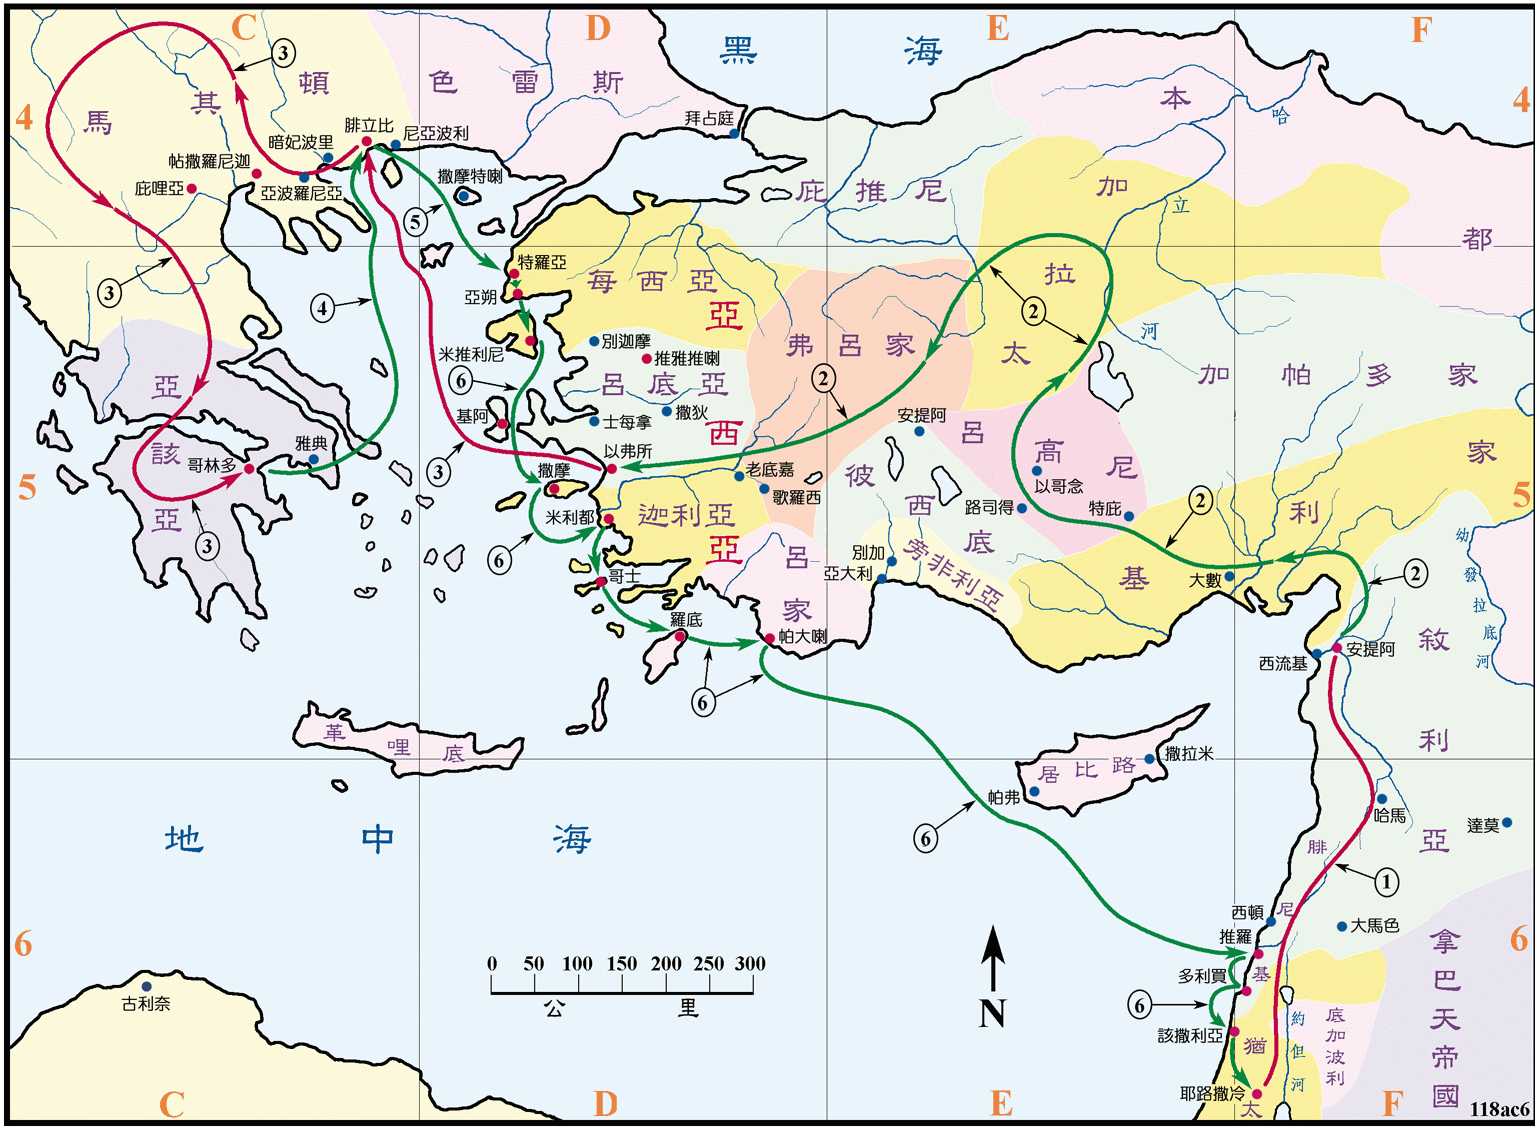
\includegraphics[width=0.9\textwidth]{ZongJie/BaoLuoShuXin/Figs/YaXiYa} 
\end{figure}












